\documentclass[tikz,border=2pt]{standalone}
\usepackage{amsmath,amssymb}
\usepackage{tikz}
\usepackage{pgfplots}
\pgfplotsset{compat=1.18}

\begin{document}
% The indifference quantity Q solves TCU2(Q) = TCU1(y_m) = 450: Q = 39.86 for the phone data.
% A threshold q between y_m = 22 and Q makes ordering q worthwhile; beyond Q keep y_m.
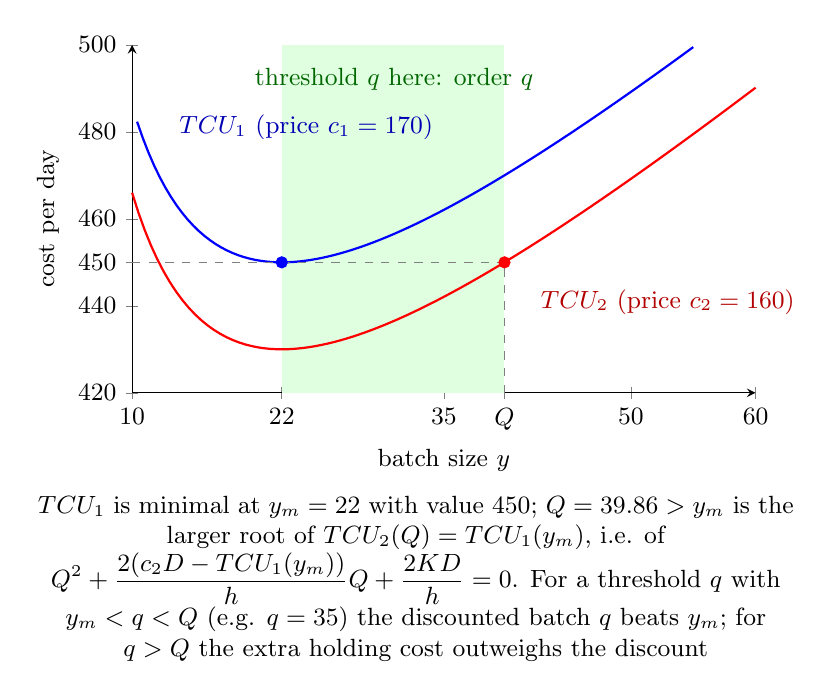
\begin{tikzpicture}
	\begin{axis}[width=9.5cm, height=6cm, xlabel={batch size $y$}, ylabel={cost per day}, xmin=10, xmax=60, ymin=420, ymax=500, axis lines=left, clip=false, tick label style={font=\small}, label style={font=\small}, samples=100, xtick={10,22,35,39.86,50,60}, xticklabels={10,22,35,$Q$,50,60}, ytick={420,440,450,460,480,500}]
		\fill[green!12] (axis cs:22,420) rectangle (axis cs:39.86,500);
		\addplot[blue, thick, domain=10.4:55] {340+1210/x+2.5*x};
		\addplot[red, thick, domain=10:60] {320+1210/x+2.5*x};
		\draw[dashed, gray] (axis cs:10,450) -- (axis cs:39.86,450);
		\draw[dashed, gray] (axis cs:39.86,420) -- (axis cs:39.86,450);
		\addplot[only marks, mark=*, mark size=2pt, blue] coordinates {(22,450)};
		\addplot[only marks, mark=*, mark size=2pt, red] coordinates {(39.86,450)};
		\node[anchor=south west, font=\small, blue!70!black] at (axis cs:13,476) {$TCU_1$ (price $c_1=170$)};
		\node[anchor=north west, font=\small, red!70!black] at (axis cs:42,446) {$TCU_2$ (price $c_2=160$)};
		\node[anchor=north, font=\small, green!40!black] at (axis cs:31,497) {threshold $q$ here: order $q$};
	\end{axis}
	\node[anchor=north, font=\small, align=flush center, text width=9.6cm] at ([yshift=-2pt]current axis.outer south) {$TCU_1$ is minimal at $y_m=22$ with value $450$; $Q=39.86>y_m$ is the larger root of $TCU_2(Q)=TCU_1(y_m)$, i.e. of $Q^2+\dfrac{2(c_2D-TCU_1(y_m))}{h}Q+\dfrac{2KD}{h}=0$. For a threshold $q$ with $y_m<q<Q$ (e.g. $q=35$) the discounted batch $q$ beats $y_m$; for $q>Q$ the extra holding cost outweighs the discount};
\end{tikzpicture}
\end{document}
